%%%%%%%%%%%%%%%%%%%%%%%%%%%%%%%%%%%%%%%%%%%%%%%%
% CHAPTER 6 -- MAIN STUDY
% METHOD
% File: tex/main-study-chapter/chapter6-main-study-METHOD.tex
%%%%%%%%%%%%%%%%%%%%%%%%%%%%%%%%%%%%%%%%%%%%%%%%
%%%%%%%%%%%%%%%%%%%%%%%%%%%%%%%%%%%%%%%%%%%%%%%%%%%%%%%%%%%%%%%%%%%%%%%%%%%%%%%%%%%%%%%%%%
% Richard Boardman PhD Thesis: Improving Tool Support for Personal Information Management
%%%%%%%%%%%%%%%%%%%%%%%%%%%%%%%%%%%%%%%%%%%%%%%%%%%%%%%%%%%%%%%%%%%%%%%%%%%%%%%%%%%%%%%%%%
%%%%%%%%%%%%%%%%%%%%%%%%%%%%%%%%%%%%%%%%%%%%%%%%%%%%%%%%%%%%%%%%%%%%%%%%%%%%%%%%%%%%%%%%%%
% NATBIB NOTES
%%%%%%%%%%%%%%%%%%%
%\citet{jon90}                ->    Jones et al. (1990) 
%   \citet[chap.~2]{jon90}       ->    Jones et al. (1990, chap. 2)
%   \citep{jon90}                ->    (Jones et al., 1990) 
%   \citep[chap.~2]{jon90}       ->    (Jones et al., 1990, chap. 2) 
%%%%%%%%%%%%%%%%%%%%%%%%%%%%%%%%%%%%%%%%%%%%%%%%%%%%%%%%%%%%%%%%%%%%%%%%%%%%%%%%%%%%%%%%%%


%%%%%%%%%%%%%%%%%%%%
%%%%%%%%%%%%%%%%%%%%
\newpage
\section{Method}
\label{main-study:method}
%%%%%%%%%%%%%%%%%%%%
%%%%%%%%%%%%%%%%%%%%%%%%%%%%%%%%%%%%%%%%%%%%%%%%%%%%%%%%%%%

%%%%%%%%%%%%%%%%%%%%%%%%%%%%%%%%%%%%%%%%%%%%%%%%%%%%%%%%%%%

%%%%%%%%%%%%%%%%%%%%
% This section describes the methodology employed in the main study as follows.
% ADD A SUMMARY. TODO TODO TODO
%%%%%%%%%%%%%%%%%%%%%%%
% Section structure
%%%%%%%%%%%%%%%%%%%%%%%
% \textbf{Section~\ref{main-study:method-choice}} discusses the challenges inherent in evaluating a PIM tool. \textbf{Section~\ref{main-study:method}} discusses the rationale behind the selection of a field study approach, and details the specific methodology employed.  Beforehand, the second objective of the main study is discussed.
\textbf{Section~\ref{main-study:method-choice}} justifies the use of a field study approach. Then \textbf{Section~\ref{main-study:method-scope}} describes the decisions made to limit the study scope. \textbf{Section~\ref{main-study:method-users}} details the study participants, and \textbf{Section~\ref{main-study:overview}} describes the 6 stages of the study.  Finally, \textbf{Section~\ref{main-study:method:data-analysis}} covers data analysis.
% The rest of \textbf{Section~\ref{main-study:method}} report the different steps of the method.

%%%%%%%%%%%%%%%%%%%%%%%%%%%%%%%%%%%%%%%%%
\subsection{Choice of Methodology}
\label{main-study:method-choice}
%%%%%%%%%%%%C%%%%%%%%%%%%%%%%%%%%%%%%%%%%
% G: This section warrants the selection of methodology for the main study.
% USE AIMS TO DRIVE THE METHOD SELECTION and JUSTIFICATION

%%%%%%%%%%%%%%%%%%%%%%%%%%%%%%%%%%%%%%%%%%%%%%%%%
% 2 types of eval: lab study and field study
%%%%%%%%%%%%%%%%%%%%%%%%%%%%%%%%%%%%%%%%%%%%%%%%%
%	\item Objective lab studies: compare between users, Objective task-centered/task-based evaluations
%	\item Field study: deep insights, Field-trial based evaluations
%%%%%%%%%%%%%%%%%%%%%%%%%%%%%%%%%%%%%%%
%%%%%%%%%%%%%%%%%%%%%%%%%%%%%%%%%%%%%%%%%%%%%%%%%%
% Consider table: lab study versus field study
%%%%%%%%%%%%%%%%%%%%%%%%%%%%%%%%%%%%%%%%%%%%%%%%%%
% However, it was also decided to be most appropriate method for evaluating WM for the following reasons:
%%%%%%%%%%%%%%%%%%%%%%%%%%%%%%%
% Selection here: Field-trial
%%%%%%%%%%%%%%%%%%%%%%%%%%%%%%%
% Choice: contextualized/fieldwork/in-situ field study
%	\item OPTIONS: choice of evaluation metrics -- Critical events/impact on "bugbears"/other problems
% Long-term data is also useful for addressing the study's second objective.
This section describes the rationale behind the selection of a field study approach.  Such an approach was clearly in line with the second objective outlined above, that of investigating user behaviour over time.  In terms of the evaluation objective, two fundamental methods were considered: (1) controlled study, or (2) field study. % Here it is argued that PIM-tools should be evaluated over the long-term within the context of real-life production activities as follows:
The author ruled in favour of a field study for the following reasons: 
% : (1) controlled studies, and (2) field studies~\cite{Dix:97}.   It was decided that a controlled study would be 




\begin{itemize}
%%%%%%%%%%%%%%%%%%%%%%%%%%%%%
% REASON 1: LONG-TERM DATA
%%%%%%%%%%%%%%%%%%%%%%%%%%%%%
% It is argued that to evaluate PIM designs properly long-term data is required. 
% Long-term data is also useful for investigating long-term issues relating to PIM.
%	\item PROS: consequences apparent only through the course of extended use, more realistic
\item Primarily, a need was ascertained to investigate the usage of WM \textit{over the long-term}.  \citet{ml:92} argue the need for a long-term perspective in the evaluation of PIM software.  They stress that the experimenter must give the participant time to get to know the features of the tool, and observe that important behaviour may take time to emerge.  They also note that a long-term study may facilitate the observation of both routine and exceptional behaviour. 

%%%%%%%%%%%%%%%%%%%%%
% REASON 2: REALISM
%%%%%%%%%%%%%%%%%%%%%
% {Situated} (own data, naturalistic, contextualized, ecological validity, insights over and beyond numbers) -- must be evaluated in work context (a la Suchman and co?). 
%	\item OPTIONS: own material/other peoples' material
\item A second concern was to carry out the investigation \textit{under realistic conditions} to maximise ecological validity.  Controlled studies have significant benefits in terms of controlling unforeseen variables, and ensuring that all participants carry out the same task, thus enabling effective comparison between them.  However in this case, the author decided that the benefits of evaluating WM \textit{in-situ}, in the context of realistic day-to-day behaviour, would be more valuable.  % In addition, the phenomena of interest -- the creation and subsequent use of folders -- would be difficult to simulate in 

\end{itemize}



%%%%%%%%%%%%%%%%%%%%%%%%%
% LINK TO CHALLENGES
%%%%%%%%%%%%%%%%%%%%%%%%%
%%%%%%%%%%%%%%%%%%%%%%%%%%%%%%%%%%%%%%%%%%%%%%%%%%%%%%
% Difficulty of evaluation
%%%%%%%%%%%%%%%%%%%%%%%%%%%%%%%%%%%%%%%%%%%%%%%%%%%%%%%%%%%%%%%%%%%%%%%%%%%%%%%%%%%%%%%
% The challenges inherent in evaluation, compounded with PIM tools.
% Compounded challenges with complex activity. Reasons why so rarely evaluated?
% Evaluation is difficult within the context of complex tasks such as PIM
% ADD: Compare with other complex activities, e.g. CSCL, user modelling (REFS)
% PIM is possibly an extreme.  Numerous methodological implications.
% Hinted at by my experiences so far -- exploratory and feasibility studies. Relate lessons from earlier chapters.
%	\item Need for appropriate evaluation criteria
%%%%%%%%%%%%%%%%%%%%%%%%%%%%%%%%%%%%%%%%%%%%%%%%%%%%%%%%%%%%%%%%%%%%%%%%%%%%%%%%%%%%%%%%%%%%%%%%%%%%%%%%%%%%%
%	lack of evaluations in PIM work, and reasons why 
%	\item Examples that have been done:
%		\item Field-work: Rodden
%		\item Laboratory: DataMountain etc., TopicShop~\cite{amento:99,amento:00}
%		\item Consider commercial practice (long-term beta trials). Although typically unpublished.
%		\item Bellotti:03, SIS:03, COntactMap?
%%%%%%%%%%%%%%%%%%%%%%%%%%%%%%%%%%%%%%%%%%%%%%%%%%%%%%%%%%%%%%%%%%%%%%%%%%%%%%%%%%%%%%
%%%%%%%%%%%%%%%%%%%%%%%%%%%%%%%%%%%%%%%%%%%%%%%%%%%%%
% \subsection{General challenges of fieldwork approach}
%%%%%%%%%%%%%%%%%%%%%%%%%%%%%%%%%%%%%%%%%%%%%%%%%%%%%
% However there are challenges associated with the field study based approach.
The author was aware of a number of challenges from the field study approach, and its application to PIM.
%%%%%%%%%%%%%%%%%
% LOGISTICS
%%%%%%%%%%%%%%%%%
% (logistics: roll-out, install, support.)
Firstly, there are \textit{logistical challenges} in installing and supporting software on peoples' desktops, and collecting feedback. 
%%%%%%%%%%%%%%%%%
% USER BUY-IN: PRIVACY
Secondly, participants may be put off by \textit{privacy concerns}. Appropriate precautions must therefore be taken by the researcher to alleviate such concerns, e.g. anonymizing all data collected. 
% ASSUMING PRIVACY NOT AN ISSUE
% This in turn raises the danger of a buggy prototype interfering with production activities and important data.   As PIM is an everyday activity, . Potential . Need for trust from users. Need for robust design that won't delete data.
Furthermore,  there may be \textit{reticence to switch from a familiar tool} to evaluate a new, un-trusted design, which may interfere with mission-critical work~\citep{Bellotti:03}. PIM plays an important part in supporting user's day-to-day roles, so any prototype being evaluated must be fully tested and robust.
%%%%%%%%%%%%%%%%%%
% INDIV DIFFS
%%%%%%%%%%%%%%%%%%
% Studies have noted how PIM behaviour and attitudes to PIM-tools varies significantly across the user population. Such individual differences must therefore be taken into account. % \textit{(also applies to studies in general)}
Another challenge results from the \textit{highly idiosyncratic} nature of PIM.  Participants may select their own tasks, or use different tool features, and it may therefore be difficult to compare between them.  The author therefore envisaged observing a wide range of behaviour.


% NO EFFECTIVE MEASURES
%%%%%%%%%%%%%%%%%%%%%%%%%%%%%
%		\item How to conceive of/define usability for tasks such as PIM?
%		\item Is usbaility an appropriate measure?
%		\item efficiency -- moving towards process (strategies and habits)
%		\item effectiveness -- moving towards outcome (achivement, result)
%		\item satisfaction -- changing towards affect ("`how does it make you feel?"').
% It is difficult to define objective usability measures for tasks such as PIM.  
% Can they be measured in terms of effectiveness and efficiency? \citet{ad:01} notes the difficulty in evaluating interactive artefacts that support complex, high-level tasks such as PIM. Particular challenges of evaluating PIM-tools include the following\footnote{NB: many of these challenges apply to studies of PIM, as well as evaluations}:
% Therefore a task-based experiment was seen as inappropriate.
% The limitations of traditional performance-based measures of usability for complex, ongoing, interleaved activities such as PIM~\citep{ad:01}, lead us to steer away from a  
% The lack of prior evaluations to follow on from meant that the work had a strong exploratory nature, and is intended as the basis for future research in this area.  A key objective of the work was to 
Further challenges resulted from the lack of accepted methodology or set of metrics for evaluating PIM tools~\citep{Whittaker-rta:00}.  This is a general problem relating to the evaluation of tools that support complex, high-level, discretionary, interleaved, activities such as PIM, where many traditional measures of usability, especially those based on efficiency and effectiveness may be inappropriate~\citep{ad:01}.  For example, in \textbf{Chapter~\ref{chapter:exploratory_study}}, several examples of ``irrational'' collecting behaviour were observed, when users collected items that they knew would never be needed again.  It is not clear how efficiency based measures can ever fully reflect the sheer range of needs that people encounter in PIM.   The difficulty in defining evaluation metrics may be a reason why few evaluations have been carried out in this area.
%%%%%%%%%%%%%%%%%%%%%%%%%%%%%%
% Exploratory approach
%%%%%%%%%%%%%%%%%%%%%%%%%%%%%%
% However Exploratory -- due to lack of previous work to build on.
% Exploratory nature due to lack of any evaluation approach, need to develop evaluation criteria
% therefore basis for further research. 
Consequently, this work had a strong exploratory nature.  \textbf{Section~\ref{main-study:overview}} reports the wide range of data collection techniques employed in this work, a key aim of which was to make recommendations regarding appropriate methodology and metrics for the evaluation of PIM software. 


%%%%%%%%%%%%%%%%%%%%%%%%%%%%%%%%%%%%%%%%%%%%%%%%%%%%%%%%%%%%%%%%%%%%%%%%%%%%%%%%%%%%%%%%%%%%%%%%%%%%%%%%%%
%%%%%%%%%%%%%%%%%%%%%%%%%%%%%%%%%%%%%%%%%%%%%%%%%%%%%%%%%%%%%%%%%%%%%%%%%%%%%%%%%%%%%%%%%%%%%%%%%%%%%%%%%%
%%%%%%%%%%%%%%%%%%%%%%%%%%%%%%%%%%%%%%%%%%%%%%%%%%%%%%%%%%%%%%%%%%%%%%%%%%%%%%%%%%%%%%%%%%%%%%%%%%%%%%%%%%
%%%%%%%%%%%%%%%%%%%%%%%%%%%%%%%%%%%%%%%%%%%%%%%%%%%%%%%%%%%%%%%%%%%%%%%%%%%%%%%%%%%%%%%%%%%%%%%%%%%%%%%%%%

%%%%%%%%%%%%%%%%%%%%%%%%%%%
% Cross-tool challenges
%%%%%%%%%%%%%%%%%%%%%%%%%%%
%%%%%%%%%%%%%%%%%%%%%%%%%%%%%%%%%%%%%%%%%%%%%%%%%%%%%
% \subsubsection{Evaluating a cross-tool design}
%%%%%%%%%%%%%%%%%%%%%%%%%%%%%%%%%%%%%%%%%%%%%%%%%%%%%
% \item Implications of cross-tool work -- further complexity and challenges.	
% Compounded again here as: 1 cross-tool feature leads to effects on multiple tools
% We are making a design intervention in 3 different tool contexts
Additional challenges resulted from evaluating a \textit{cross-tool} design such as WM.  
Typically evaluations assess the impact of a new tool design in the context of user tasks centred on that specific tool.  However, as a PIM-integration mechanism, WM affects the operation of three distinct PIM-tools: files, email, and bookmarks.  Therefore, the installation of WM, although one piece of software, causes a design intervention in three different tool contexts.  All three interventions must therefore be taken into consideration during evaluation.  % There may also be inter-dependencies between the tools to be taken into consideration.
% THINK: extract key points to expand here}. Impact on choice of method

%%%%%%%%%%%%%%%%%%%%%%%%%%%%%%%%%%%%%%%%%%%%%%%%%%%%%%%%%%%%%%%%%%%%%%%%%%%%%%%%%%%%%%%%%%%%%%%%%%%%%%%%%%
%%%%%%%%%%%%%%%%%%%%%%%%%%%%%%%%%%%%%%%%%%%%%%%%%%%%%%%%%%%%%%%%%%%%%%%%%%%%%%%%%%%%%%%%%%%%%%%%%%%%%%%%%%
%%%%%%%%%%%%%%%%%%%%%%%%%%%%%%%%%%%%%%%%%%%%%%%%%%%%%%%%%%%%%%%%%%%%%%%%%%%%%%%%%%%%%%%%%%%%%%%%%%%%%%%%%%
%%%%%%%%%%%%%%%%%%%%%%%%%%%%%%%%%%%%%%%%%%%%%%%%%%%%%%%%%%%%%%%%%%%%%%%%%%%%%%%%%%%%%%%%%%%%%%%%%%%%%%%%%%


	
%%%%%%%%%%%%%%%%%%%%%%%%%%%%%%%%%%%%%%%
\subsection{Study Scope}
\label{main-study:method-scope}
%%%%%%%%%%%%%%%%%%%%%%%%%%%%%%%%%%%%%%%
% THINK: here or method?
% still somewhat unrealistic but still more realistic than most. 
% They were similar to those applied to the exploratory study in \textbf{Chapter~\ref{chapter:exploratory_study}}:
Several constraints were applied to the study to compensate for its ambitious scope (both cross-tool and longitudinal), and the limited manpower resources available:
\begin{itemize}

% i.e. the study did not consider the extended personal information environment beyond one single computer.
\item \textit{One computer per participant } -- As in the exploratory study, a focus was taken on PIM performed in each participant's self-nominated primary work computer.


%%%%%%%%%%%%%%%%%%%%
% 3 collections
%%%%%%%%%%%%%%%%%%%%
\item \textit{Three collections of personal information: files, email and bookmarks} -- The study focused on the three PIM-tools influenced by WM.  

% extent of the file system which was included.
% One scoping extension was made in the file system relative to the exploratory study where several participants mentioned using   In this study, multiple areas were tracked if they were used to manage personal files by the participant concerned.
\item \textit{One area of the personal file system} -- WM was limited on monitoring one area of the file system, nominated by the participant as their primary location for storing personal documents, e.g. ``My Documents''.  Likewise, a decision was taken to focus the study on the same area of the file system.  However, 
two participants (F3 and M7) actively managed files in two locations.  In their cases, both areas were covered by the study.

Furthermore, as in the exploratory study, areas of the monitored portion of the file system which contained source code, temporary files, and program executables were omitted from the data analysis.  

\end{itemize}


%%%%%%%%%%%%%%%%%%%%%%%%%%%%%%%%%%%%%%%%%%%%%%%%%%%%%%%%%%%%%%%%%%%%%%%%%%%%%%%%%%%%%%%%%%%%%%%%%%%%%%%%%%
%%%%%%%%%%%%%%%%%%%%%%%%%%%%%%%%%%%%%%%%%%%%%%%%%%%%%%%%%%%%%%%%%%%%%%%%%%%%%%%%%%%%%%%%%%%%%%%%%%%%%%%%%%
%%%%%%%%%%%%%%%%%%%%%%%%%%%%%%%%%%%%%%%%%%%%%%%%%%%%%%%%%%%%%%%%%%%%%%%%%%%%%%%%%%%%%%%%%%%%%%%%%%%%%%%%%%
%%%%%%%%%%%%%%%%%%%%%%%%%%%%%%%%%%%%%%%%%%%%%%%%%%%%%%%%%%%%%%%%%%%%%%%%%%%%%%%%%%%%%%%%%%%%%%%%%%%%%%%%%%


%%%%%%%%%%%%%%%%%%%%%%%%%%%%%%%
\subsection{Participants}
\label{main-study:method-users}
%%%%%%%%%%%%%%%%%%%%%%%%%%%%%%%
% OPTION: frame user selection as intentional?


%%%%%%%%%%%%%%%%%%%%%%%%%%%%%%%%%%%%%%%%
% CHOICE OF COLLAGUES
% Reasons for selecting colleagues
%%%%%%%%%%%%%%%%%%%%%%%%%%%%%%%%%%%%%%%%
% ADD: selection absed on PIM-tools?
% Reasons for choosing colleagues: upsides and downsides. 
% Consideration of other options.  
% Compare with experiences of other researchers: Bellotti's difficulties, Whittaker.
Eight colleagues of the author were selected to take part in the study.  \textbf{Table~\ref{table:main-study:participants}} summarizes their details.
The use of colleagues as participants is justified as follows.
Firstly, it was hoped that the study could leverage the existing trust basis between the researcher and his colleagues -- avoiding possible privacy problems of working with strangers' personal data.
Secondly, they were all technologically aware and ready to work with beta software.
% Participants gave themselves an average technical expertise self-rating of  6 out of 7 in the profiling interview questionnaire.
A third reason was pragmatic: it was easy to meet with them to carry out interviews, and install software.

%%%%%%%%%%%%%%%%%%%%%
% REASONS AGAINST
%%%%%%%%%%%%%%%%%%%%%
% ADD: how was these obviated.  
Two methodological problems result from this set of participants.  Firstly, since they already knew the researcher, there is the possibility of potential bias in favour of WM.  To try and counter this, participants were asked to be unbiased and honest in their feedback. The wide range of feedback received on WM -- both positive and negative -- suggests that this was achieved.  Additionally, the small number of participants meant that the results are unlikely to be applicable to the wider population of computer users.  However, the intention was to produce interesting, indicative results, and to highlight routes for follow-up research. Overall, it is argued that the above benefits outweigh these downsides.   %, and that the study is a worthwhile piece of work 

%%%%%%%%%%%%%%
% 2 TRACKS
%%%%%%%%%%%%%%
The eight participants were grouped into two groups as follows:
\begin{itemize}
% Participants F1 through F4 moved onto the main study after taking part in the initial evaluation of WM as reported in \textbf{Chapter~\ref{chapter:design}}. 
\item \textit{Track 1} -- The first four participants (identified as F1--F4) had previously taken part in the 
initial evaluation reported in \textbf{Chapter~\ref{chapter:design}}.  In addition, participants F1 and F2 had also taken part in the exploratory study in \textbf{Chapter~\ref{chapter:exploratory_study}} as participants P1 and P2 respectively.
  
\item \textit{Track 2}: the second four participants (identified as M5--M8) had not participated in any earlier investigations by the author.
\end{itemize}




%%%%%%%%%%%%%%%%%%%%%%%%%%%%%%%%%%%%%%%%%%%%%
% ADD?: link to installation problems stuff
%%%%%%%%%%%%%%%%%%%%%%%%%%%%%%%%%%%%%%%%%%%%%

%%%%%%%%%%%%%%%%%%%%%%%%%%%%%%%%%%%%%%%%%%
% ADD: siogn-posting to next section?
%%%%%%%%%%%%%%%%%%%%%%%%%%%%%%%%%%%%%%%%%%
% The field-study methodology is described in detail in the next section.

%%%%%%%%%%%%%%%%%%%%%%%%%%%%%%%%%%%%%%%%%
% TABLE OF PARTICIPANTS IN MAIN STUDY
%%%%%%%%%%%%%%%%%%%%%%%%%%%%%%%%%%%%%%%%%
\begin{sidewaystable}
\begin{center}
\begin{footnotesize}
\setlength{\extrarowheight}{2pt}
% Table generated by Excel2LaTeX from sheet 'MAIN STUDY PHASE 2'
\begin{tabular}{|p{1.6cm}|p{1.7cm}|p{1.7cm}|c|c|c|p{1.4cm}|p{1cm}|p{1cm}|p{1cm}|c|}
\hline
{\bf Main Study  ID} & {\bf ID in Exp. Study (see Ch.~\ref{chapter:exploratory_study})} & {\bf ID in Initial eval. (see Ch.~\ref{chapter:design})} &  {\bf Age} &  {\bf Sex} & {\bf Job Role} & {\bf Operating System} & {\bf \# file folders} & {\bf \# email folders } & {\bf \# BM folders } & {\bf Cross-tool profile} \\
\hline
        F1 &         P1 &         F1 &      35-40 &          M & Researcher &    Win2000 &         33 &         50 &          3 & CT2 (F1, E2, B2) \\
\hline
        F2 &         P2 &         F2 &      20-25 &          M &    Student &    Win2000 &        128 &         41 &         55 & CT1 (F1, E2, B1) \\
\hline
        F3 &          - &         F3 &      30-35 &          F &    Student &      WinXP &        139 &         10 &          7 & CT3 (F1, E3, B2) \\
\hline
        F4 &          - &         F4 &      20-25 &          M &    Student &      WinXP &         31 &         33 &        196 & CT1 (F2, E2, B1) \\
\hline
        M5 &          - &    {\bf -} &      25-30 &          M &    Student &    Win2000 &         59 &         20 &         11 & CT2 (F2, E2, B2) \\
\hline
        M6 &          - &          - &      20-25 &          M &    Student &    Win2000 &        235 &         10 &          6 & CT1 (F1, E1, B1) \\
\hline
        M7 &          - &          - &      25-30 &          M &    Student &    Win2000 &         28 &          6 &          0 & CT3 (F2, E3, B3) \\
\hline
        M8 &          - &          - &      30-35 &          M & Researcher &    Win2000 &         69 &         10 &         26 & CT3 (F2, E3, B3) \\
\hline
   Average &            &            &            &            &            &            &       90.3 &       22.5 &       38.0 &            \\
\hline
\end{tabular}  
\end{footnotesize}
\caption{Participants in the main study}
\label{table:main-study:participants}
\end{center}
\end{sidewaystable}
\normalsize



%%%%%%%%%%%%%%%%%%%%%%%%%%%%%%%%%%%%%%%%%%%%%%%%%%%%%%%%%%%%%%%%%%%%%%%%%%%%%%%%%%%%%%%%%%%%%%%%%%%%%%%%%%
%%%%%%%%%%%%%%%%%%%%%%%%%%%%%%%%%%%%%%%%%%%%%%%%%%%%%%%%%%%%%%%%%%%%%%%%%%%%%%%%%%%%%%%%%%%%%%%%%%%%%%%%%%
%%%%%%%%%%%%%%%%%%%%%%%%%%%%%%%%%%%%%%%%%%%%%%%%%%%%%%%%%%%%%%%%%%%%%%%%%%%%%%%%%%%%%%%%%%%%%%%%%%%%%%%%%%
%%%%%%%%%%%%%%%%%%%%%%%%%%%%%%%%%%%%%%%%%%%%%%%%%%%%%%%%%%%%%%%%%%%%%%%%%%%%%%%%%%%%%%%%%%%%%%%%%%%%%%%%%%


	

%%%%%%%%%%%%%%%%%%%%%%%%%%%%%%%%%%%%%%%%%%%%%%
\subsection{Study Process}
\label{main-study:overview}
%%%%%%%%%%%%%%%%%%%%%%%%%%%%%%%%%%%%%%%%%%%%%%

%%%%%%%%%%%%%%%%%%%%%%%%%%
% OVERVIEW OF METHOD
% participants proceeded onto Phase 2 of the study in which we tracked the evolution of the three collections over time.  The average participation was 286 days (CHECK).
%%%%%%%%%%%%%%%%%%%%%%%%%%
The study process consisted of six stages, as illustrated in \textbf{Figure~\ref{fig:main-study:method-overview}}:
\begin{enumerate}
% STAGE 1
\item Initial profile interview \textit{(all participants)}.
% STAGE 2
\item \textit{Pre-WM} tracking \textit{(track 2 participants only)}.
% STAGE 3
\item Interim interview and installation of WM \textit{(all participants)}
% STAGE 4
\item \textit{With-WM} tracking, with WM installed \textit{(all participants)}.
% STAGE 5
\item Closing interview and uninstall of WM \textit{(all participants)}.
%%%%%%%%%%%%%%%%%%%
% T+6 tracking
%%%%%%%%%%%%%%%%%%%
% STAGE 6
\item \textit{Post-WM} tracking \textit{(all participants)}.
\end{enumerate}

%%%%%%%%%%%%%%%%%%%%%%%%%%%%%%%%%%%%%%
% %%%%%%%%%%%%%%%%%%%%%%%%%%%%%%%%%%%%
% FIGURE - Main Study Process Overview
% %%%%%%%%%%%%%%%%%%%%%%%%%%%%%%%%%%%%
%%%%%%%%%%%%%%%%%%%%%%%%%%%%%%%%%%%%%%
\begin{figure}[t]
	\begin{center}
		\leavevmode
		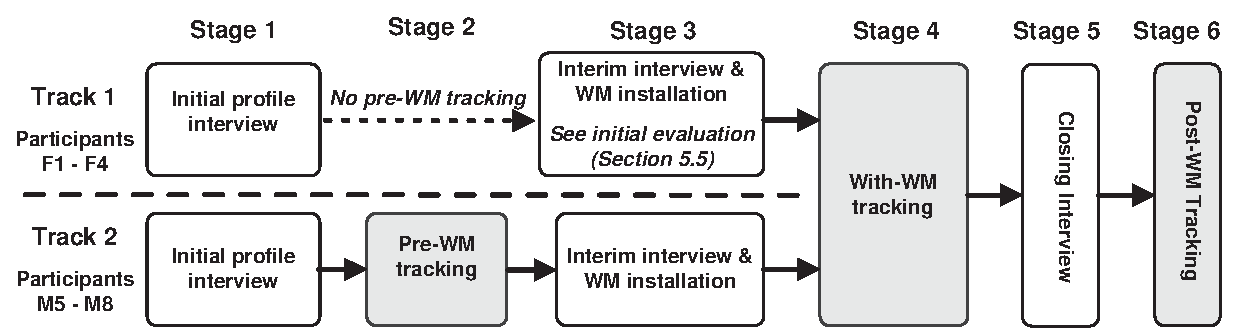
\includegraphics[width=\textwidth]{pictures/main-study/main-study-method.pdf}
	\end{center}
	\caption{Main Study: overview of method}
	\label{fig:main-study:method-overview}
\end{figure}

%%%%%%%%%%%%%%%%%%%%%%%%%%%%%%%%%%%%%
% MUST EXPLAIN TWO TRACKS CLEARLY
% Or consider merging!
%%%%%%%%%%%%%%%%%%%%%%%%%%%%%%%%%%%%%
% Eight participants took part in the study, during which WE tracked the evolution of the three collections and the strategies used to manage them. Participation was divided across two different tracks:
\textbf{Figure~\ref{fig:main-study:method-overview}} shows how the two tracks differed in terms of their participation in the various stages of the study.  In summary, the track 1 participants did not take part in stage 2 (pre-WM tracking), as stages 1 and 3 (the initial and interim interviews) were combined in the initial evaluation reported in \textbf{Chapter~\ref{chapter:design}}.  Therefore they proceeded straight on to stage 4.  \textbf{Table~\ref{table:main-study:participation}} provides a detailed breakdown of participation on an individual basis.

%%%%%%%%%%%%%%%%%%%%%%%%%%%%%%%%%%%%%%%%%
% Multiple methods of data collection
%%%%%%%%%%%%%%%%%%%%%%%%%%%%%%%%%%%%%%%%%
% to reduce inappropriate certainty, and enhance interpretability. 
% TODO: emphasise exploratory nature more?
% Report difficulty in diaries
Throughout the study, data was collected through a range of methods including interviews, diary and logging.  A range of methods were employed for two reasons.  Firstly, it was envisaged that their triangulation would help build a rich picture of participants' behaviour. 
%For instance, it was hoped that the log data would act as a reference during the interviews.
Secondly, the author also had an interest in exploring the worth of each method.
% triangulation
% The multiple data sources were triangulated as described in \textbf{Section~\ref{main-study:method:triangulation}}. 

The following sections discuss each stage of the study in more detail.
% Refer to experimental material in appendix (eg. q'aire). 
Copies of the experimental materials are included in \textbf{Appendix~\ref{chap:appendices-main-study-material}}. % \textit{NB: need to mention that F1--F4 had a different profiling questionnaire?}




%%%%%%%%%%%%%%%%%%%%%%%%
% STAGE 1: PROFILING
%%%%%%%%%%%%%%%%%%%%%%%%
%%%%%%%%%%%%%%%%%%%%%%%%%%%%%%%%
\subsubsection{Stage 1: Initial Interview (all participants)}
%%%%%%%%%%%%%%%%%%%%%%%%%%%%%%%%
% Much as per Chapter 4, avoid big repeat. 
% Need to repeat: Prelims (e.g. disclosure agreement)
% Need detail on interview structure: background expertise, general survey of computer usage, how organized do you consider yourself?, guided tour (practices, satisfaction, integration with other tools), todo items, change anything. Also asked about requirements for integration.
% Questionnaire design?  See appendix.
The initial interview followed a similar format to that employed in the exploratory study in \textbf{Chapter~\ref{chapter:exploratory_study}}\footnote{Profiling interviews were not carried out for participants F1 and F2 since they had already taken part in the exploratory study.}.  Participants were asked about their PIM practices regarding files, email and bookmarks in turn.   An additional question was added regarding views on existing levels of integration between the three PIM-tools.  Note that the privacy precautions outlined in \textbf{Chapter~\ref{chapter:exploratory_study}} were also followed here.
% Regarding WorkspaceMirror, not told (too much) about nature of tool in advance
Studies were carried out in the work environment of the participant and took about one hour.  All interviews were recorded on mini-disc and fully transcribed.

In the exploratory study, folder structures had been recorded via a screenshot and transcribed by hand.  To automate this process in the main study, a tool called \textit{WorkspaceSnapper} (WS) was developed by the author.  WS recorded the file, email and bookmark folder structures as a text file, along with counts of items within folders.  To limit intrusion, details of specific items -- such as filenames -- were not recorded.  During the interview, WS was installed and used to obtain snapshots of the initial folder structures.  Participants were shown the resulting text file to alleviate any privacy concerns. After the profiling interview,  WS was left installed.

%Analysis: organizational dimensions, cross-tool profiling as in \textbf{Chapter~\ref{chapter:exploratory_study}}.  
%Starting point for workspace evaluation transcript.
% Data analysis is described in \textbf{Section~\ref{main-study:method:triangulation}}




%%%%%%%%%%%%%%%%%%%%%%%%
% STAGE 2: PHASE 1
%%%%%%%%%%%%%%%%%%%%%%%%
%%%%%%%%%%%%%%%%%%%%%%%%%%%%%%%%%%%%%%%
\subsubsection{Stage 2: Pre-WM Tracking (track 2 participants only)}
%%%%%%%%%%%%%%%%%%%%%%%%%%%%%%%%%%%%%%%
% Refer to experimental material in appendix (eg. q'aire)
The PIM practices of the four \textit{track 2} participants (M5--M8) were observed over several weeks \textit{before} WM was installed\footnote{The track 1 participants were directly exposed to WM during the initial evaluation reported in \textbf{Chapter~\ref{chapter:design}}, and therefore did not take part in stage 2.}.  This was done to characterise their ``normal'' PIM behaviour, and so better ascertain the effect of the design intervention. Average participation in stage 2 was 57 days (min: 32, max: 75, SD: 21.6).  Multiple methods of data collection were employed to help build up a rich picture of participants' behaviour:

\begin{itemize}
%%%%%%%%%%%%%
% Snapshots
%%%%%%%%%%%%%
\item \textit{Snapshots of the three folder structures} -- Participants were asked to manually initiate snapshots using WorkspaceSnapper to lessen the infringement of their privacy.  Snapshots were requested via email at two-week intervals. % returned as zipped email

%%%%%%%%%%%
% DIARY
%%%%%%%%%%%
\item \textit{Diary} -- Participants were also asked to keep a diary of significant incidents relating to the management of the three collections. Two incidents were provided as examples: (1) creating a new folder, and (2) failing to locate an item.  % The diary template is shown in \textbf{Appendix~\ref{chap:appendices-main-study-material}}.

\end{itemize}


%%%%%%%%%%%%%%%%%%%%%%%%%%
% AVERAGE PARTICIPATION
%%%%%%%%%%%%%%%%%%%%%%%%%%














%%%%%%%%%%%%%%%%%%%%%%%%
% STAGE 3: DESIGN INTERVENTION
%%%%%%%%%%%%%%%%%%%%%%%%
%%%%%%%%%%%%%%%%%%%%%%%%%%%%%%%%%%%%%%%%%%%%%%%%%%%%%%%%%%%
\subsubsection{Stage 3: Interim Interview (all participants)}
%%%%%%%%%%%%%%%%%%%%%%%%%%%%%%%%%%%%%%%%%%%%%%%%%%%%%%%%%%
% Design as an intervention in the study process.  
% interim interview + installation
%%%%%%%%%%%%%%%%%%%%%%%%%%%%%%%%%%%%%%

The \textit{track 2} participants then took part in a 30 minute interim interview\footnote{For the \textit{track 1 participants}, this stage was reported in the initial evaluation in \textbf{Chapter~\ref{chapter:design}}.}. Firstly, they were questioned regarding major events in the three collections of personal information over stage 2.  A transcript of folder changes and diary events was used as a shared resource in the interview (see \textbf{Section~\ref{main-study:method:data-analysis}}).
% showed how to create and delete a folder
Then, WM was installed on their machines, folder-mirroring was demonstrated by the author, and the participants were asked for their first impressions.

% \textit{Consider moving to next section}.
It was difficult to find users with a set of PIM-tools that were fully compatible with WM, and many potential participants had to be ruled out. \textbf{Table~\ref{table:main-study:participants-problems}} summarizes the incompatibilities encountered for the final participants which limited the extent of mirroring. In each case, they were asked to consider whether they would have mirrored events, and if so, to perform mirroring manually.
% These were primarily due to two reasons: (1) the wide range of PIM-tools in use, and (2) the relative immaturity of the prototype.
Participant M5 stored his personal files on a UNIX-based network drive which was incompatible with the file-monitoring capabilities of WM.  % of the \texttt{dotNetWatcher} component of 
Participants M3 and M7 managed files in two areas of the file system, whilst WM was limited to monitoring one area.  M4 and M5 used MS Outlook Express to manage email, rather than MS Outlook as required by WM.  M5 switched to MS-Outlook before installing WM, as he reported planning to do for some time.
%%%%%%%%%%%%%%%%%%%%%%%%%%%
% Installation problems
%%%%%%%%%%%%%%%%%%%%%%%%%%%
% As mentioned above, installation problems were encountered  (see \textbf{Table~\ref{table:main-study:participants-problems}}). 

%%%%%%%%%%%%%%%%%%%%%%%%%%%%%%%%%%%%%%%%%
% TABLE OF INSTALLATION PROBLEMS
%%%%%%%%%%%%%%%%%%%%%%%%%%%%%%%%%%%%%%%%%
\begin{table}[hbtp]
\begin{center}
\begin{footnotesize}
\setlength{\extrarowheight}{2pt}
\begin{tabular}{|c|p{4cm}|p{5cm}|p{2.4cm}|}
% Table generated by Excel2LaTeX from sheet '3 Installation problems'
\hline
  {\bf Participant} & {\bf File-related problems} & {\bf Email-related problems} & {\bf Bookmark-related problems} \\
\hline
        F1 &          - &          - &          - \\
\hline
        F2 &          - &          - &          - \\
\hline
        F3 & Personal files split over two areas of the file system (Desktop and My Documents) &          - &          - \\
\hline
        F4 &          - & Use of MS-Outlook Express (incompatible with WM) &          - \\
\hline
        M5 & Use of  network drive (incompatible with WM) & Use of MS-Outlook Express (incompatible with WM). User agreed to switch to MS-Outlook. &          - \\
\hline
        M6 &          - &          - &          - \\
\hline
        M7 & Personal files split over two areas of the file system (My Documents and `D' drive) &          - &          - \\
\hline
        M8 &          - &          - &          - \\
\hline
\end{tabular}  
\end{footnotesize}
\caption{WM installation problems: incompatibilities with PIM-tools}
\label{table:main-study:participants-problems}
\end{center}
\end{table}
\normalsize








%%%%%%%%%%%%%%%%%%%%%%%%
% STAGE 4: PHASE 2
%%%%%%%%%%%%%%%%%%%%%%%%
%%%%%%%%%%%%%%%%%%%%%%%%%%%%%%%%%%%%%%%%%%%%%%%%%%%%
\subsubsection{Stage 4: With-WM Tracking (all participants)}
%%%%%%%%%%%%%%%%%%%%%%%%%%%%%%%%%%%%%%%%%%%%%%%%%%%

The next stage involved the tracking of participants' PIM practices with WM installed. Average usage of WM was 44 days (min: 16, max: 93, SD: 50.4, see \textbf{Table~\ref{table:main-study:participation}} for more detail).

%%%%%%%%%%%%%%%%%%%%%%%%%%%%%%%%%%%%%%%%%%%%%%%%%%%%%%%%%
% Data collection: diary and log/snapshots as before
%%%%%%%%%%%%%%%%%%%%%%%%%%%%%%%%%%%%%%%%%%%%%%%%%%%%%%%%%
% Refer to experimental material in appendix (eg. q'aire)
Both methods of data collection from stage 2 were employed: (1) bi-weekly snapshots of the three folder structures captured with WS, and (2) a diary of significant events.  Additionally, two other forms of data collection were used.  Firstly, occasional interviews were carried out to check WM was working satisfactorily, and to get feedback. Secondly, WM maintained a log of mirroring events.  % During data analysis, data was triangulated into the workspace evolution transcript (see \textbf{Section~\ref{main-study:method:triangulation}}).
Apart from the early version used in the feasibility study, WM was robust and did not crash.  By default, WM was started automatically at start-up, and most participants left it running continuously whilst their computer was switched on.  % The next section focuses on the feedback obtained regarding the design of WM, rather than implementation details.


% as in Stage 2

%%%%%%%%%%%%%%%%%%%%%%%%
% STAGE 5: CLOSING INTERVIEW
%%%%%%%%%%%%%%%%%%%%%%%%
%%%%%%%%%%%%%%%%%%%%%%%%%%%%%%%%%%%%%%%%%%%%%%%%%%%
\subsubsection{Stage 5: Closing Interview (all participants)}
%%%%%%%%%%%%%%%%%%%%%%%%%%%%%%%%%%%%%%%%%%%%%%%%%%%

In the closing interview, participants were asked for feedback on the WM prototype via a series of questions addressing impact on file, email and bookmark management in turn.  % Participants were able to comment on any aspect of the design.
Secondly, participants were asked about changes to their PIM strategies over the course of the study to date, and what factors had influenced those changes.  Finally, WM was uninstalled from their computer\footnote{Participant F2 requested to keep WM, and continued to use it for 80 days after the study had finished}.  % A full copy of the closing interview can be seen in \textbf{Appendix~\ref{chap:appendices-main-study-material}}. % textit{NB: need to mention that different participants had different forms of the questionnaire?}


% appendix


%%%%%%%%%%%%%%%%%%%%%%%%%%%%%%%%%%%%%
% Refer to materials in appendix?
%%%%%%%%%%%%%%%%%%%%%%%%%%%%%%%%%%%%%

%%%%%%%%%%%%%%%%%%%%%%%%
% STAGE 6: CLOSING INTERVIEW
%%%%%%%%%%%%%%%%%%%%%%%%
%%%%%%%%%%%%%%%%%%%%%%%%%%%%%%%%%%%%%%%%%%%%%%%%%%%
\subsubsection{Stage 6: Post-WM Tracking (all participants)}
%%%%%%%%%%%%%%%%%%%%%%%%%%%%%%%%%%%%%%%%%%%%%%%%%%%

Approximately six months after the closing interview, participants were requested for a final snapshot using WS, after which it was uninstalled.

%%%%%%%%%%%%%%%%%%%%%%%%%%%%%%
% TABLE OF PARTICIPATION
%%%%%%%%%%%%%%%%%%%%%%%%%%%%%%
%%%%%%%%%%%%%%%
% TO PLACE
%%%%%%%%%%%%%%%
% MOVE TO METHOD/RESULTS
% All eight participants in the field study reported in this chapter installed and used WM within their day-to-day workspace for an average of 69 days (range: 16 to 143). 
Average total participation was 286 days (min 218, max 309, SD: 32.2). Participation in the different stages of the study varied between participants and is summarized in \textbf{Table~\ref{table:main-study:participation}}.

% \textbf{Table~\ref{table:main-study:participation}} provides more detail on participation in the six stages.

% The following sections discuss each stage of the study in more detail.


%%%%%%%%%%%%%%%%%%%%%%%%%%%%%%%%%%%%%%%%%%%%%%%%%%%
% TABLE X: STUDY PARTICIPATION PER PARTICIPANT
%%%%%%%%%%%%%%%%%%%%%%%%%%%%%%%%%%%%%%%%%%%%%%%%%%%
% Also consider table in Bellotti et al 2003
% Participation in the various stages of the study varied between participants as described in \textbf{Table~\ref{table:main-study:participation}}.
\begin{sidewaystable}% [hbtp]
\begin{center}
\begin{footnotesize}
\setlength{\extrarowheight}{2pt}
% Table generated by Excel2LaTeX from sheet 'Participation'
\begin{tabular}{|c|p{2cm}|p{2cm}|p{2cm}|p{2cm}|p{2cm}|p{2cm}|p{2.5cm}|}
\hline
{\bf Participant} & {\bf Stage 1: Initial interview} & {\bf Stage 2: Pre-WM tracking (\# days)} & {\bf Stage 3: Interim interview and WM installation} & {\bf Stage 4: With-WM tracking (\# days)} & {\bf Stage 5: Closing interview} & {\bf Stage 6: Post-WM tracking} & {\bf Total participation (\# days) } \\
\hline
F1 (track 1) & \checked (see exploratory study, \textbf{Chapter~\ref{chapter:exploratory_study}}) &          - & \checked (see initial evaluation in \textbf{Chapter~\ref{chapter:design}}) &         57 &   \checked &   \checked &        260 \\
\hline
F2 (track 1) & \checked (see exploratory study, \textbf{Chapter~\ref{chapter:exploratory_study}}) &          - & \checked (see initial evaluation in \textbf{Chapter~\ref{chapter:design}}) &        120 &   \checked &   \checked &        309 \\
\hline
F3 (track 1) &   \checked &          - & \checked (see initial evaluation in \textbf{Chapter~\ref{chapter:design}}) &        143 &   \checked &   \checked &        309 \\
\hline
F4 (track 1) &   \checked &          - & \checked (see initial evaluation in \textbf{Chapter~\ref{chapter:design}}) &        111 &   \checked &   \checked &        305 \\
\hline
M5 (track 2) &   \checked &         32 &   \checked &         65 &   \checked &   \checked &        219 \\
\hline
M6 (track 2) &   \checked &         75 &   \checked &         18 &   \checked &   \checked &        302 \\
\hline
M7 (track 2) &   \checked &         75 &   \checked &         16 &   \checked &   \checked &        306 \\
\hline
M8 (track 2) &   \checked &         46 &   \checked &         20 &   \checked &   \checked &        281 \\
\hline
{\bf Average (\#days)} &          - &         57 &          - &      68.75 &          - &          - &        286 \\
\hline
\end{tabular}  
\end{footnotesize}
\caption{Summary of participation in each stage of the main study}
\label{table:main-study:participation}
\end{center}
\end{sidewaystable}
\normalsize

%%%%%%%%%%%%%%%%%%%%%%%%%%%%%%%%%%%%%%%%%%%%%%%%%%%%%%%%%%%%%%%%%%%%%%%%%%%%%%%%%%%%%%%%%%%%%%%%%%%%%%%%%%
%%%%%%%%%%%%%%%%%%%%%%%%%%%%%%%%%%%%%%%%%%%%%%%%%%%%%%%%%%%%%%%%%%%%%%%%%%%%%%%%%%%%%%%%%%%%%%%%%%%%%%%%%%
%%%%%%%%%%%%%%%%%%%%%%%%%%%%%%%%%%%%%%%%%%%%%%%%%%%%%%%%%%%%%%%%%%%%%%%%%%%%%%%%%%%%%%%%%%%%%%%%%%%%%%%%%%
%%%%%%%%%%%%%%%%%%%%%%%%%%%%%%%%%%%%%%%%%%%%%%%%%%%%%%%%%%%%%%%%%%%%%%%%%%%%%%%%%%%%%%%%%%%%%%%%%%%%%%%%%%

%%%%%%%%%%%%%%%%%%%%%%%%
% DATA ANALYSIS
%%%%%%%%%%%%%%%%%%%%%%%%
%%%%%%%%%%%%%%%%%%%%%%%%%%%%%%%%%%%%%%%%%%%%%%%%%%%
\subsection{Data Analysis}
\label{main-study:method:data-analysis}
%%%%%%%%%%%%%%%%%%%%%%%%%%%%%%%%%%%%%%%%%%%%%%%%%%%
% Include: Learning from lessons of previous studies?

% % Four of our colleagues have been using WorkspaceMirror in their primary desktop workspaces over four months, and are providing feedback via diaries and weekly interviews.  WE have also correlated this qualitative data with fortnightly logs of their evolving folder hierarchies to track their usage of any mirrored folders.  WE triangulated the data to build up a rich picture of the user's attitude to WorkspaceMirror, and investigate whether it influenced their PIM practices.  
% Mass of data collected via the range of methods. Data overload!
% Data includes interviews, logs, and diaries from both before and after installation of WM.
% The preceding section describes how data was collected via a range of techniques to build up a rich picture of participants' PIM practices.
% This section discusses how the different forms of study data were processed and collated.

%%%%%%%%%%%%%%%%%%%%%%%%%%%%%%%%%%%%%%%%%
% ADD: whatabout questionnaire data?
%%%%%%%%%%%%%%%%%%%%%%%%%%%%%%%%%%%%%%%%%

%%%%%%%%%%%%%%%%%%%%%%%%%%%%%%%%%%%%%%%%
% content analsysi of interview data
% Extraction of critical incidents, most frequent and important issues and problems
% Quote extraction to illustrate main themes.
% to give idea of PIM behaviour (pre and post design intervention, and also usage of WM tool). 
%%%%%%%%%%%%%%%%%%%%%%%%%%%%%%%%%%%%%%%% 
% Content analysis was performed through a process of affinity clustering (CLARIFY).  Key themes were extracted and used to produce a coding scheme.  This was then applied across all participants.  Particular attention was paid to issues relating to WM, and to longitudinal PIM issues.
% Need to report to where it is reported?
All interview and diary data was transcribed into one text file for each participant.  An initial coding scheme was developed relating to areas of key interest: (1) feedback on WM, and (2) comments relating to changes in strategy.  The coding scheme was iteratively applied to the data, and extended with additional interesting themes that came to light.  A sample of the qualitative data collected is shown in \textbf{Appendix~\ref{chap:appendices--study-data}} on page~\pageref{chap:appendices--study-data:main-study}.

%%%%%%%%%%%%%%%%%%%%%%%%%%%%%%%%%%%%%%%%%%%%%%
% Analysis of folder structure snapshots
% Repeat of analyses from exploratory study, including folder overlap?
%%%%%%%%%%%%%%%%%%%%%%%%%%%%%%%%%%%%%%%%%%%%%%
The folder snapshots recorded in stage 1 were analysed in terms of \textit{organizational dimensions}, and \textit{folder overlap}.  Participants' organizing strategies were also characterized, and a cross-tool profile produced.  Please see \textbf{Chapter~\ref{chapter:exploratory_study}} for detail on these three techniques.
% Each participant's cross-tool profile was also collated based on their three tool-specific organizing strategies (see \textbf{Table~\ref{table:main-study:participants}}).

%%%%%%%%%%%%%%%%%%%%%%%
% Compilation of Workspace Evolution Transcript WET
%%%%%%%%%%%%%%%%%%%%%%%
% Triangulation of longitudinal data -- within Workspace Evolution Transcript, the collation of data from multiple methods between different data sources (objective and subjective). 
% Focus on monitored areas, but where users files split between multiple areas, took those into account.
All longitudinal data was collated into a \textit{workspace evolution transcript} (WET) for each participant. The WET included the following pieces of information:
\begin{itemize}
% evolution of folder structures and number of items. 

\item \textit{Incremental changes to the folder structures} -- These were identified manually for each of the three PIM-tools. Changes in the overall number of folders and unfiled items were also calculated to ascertain the growth of the collections.

\item \textit{Folder-related events} -- Events such as folder creation were identified and annotated with any relevant diary or interview comments.

\item \textit{Other events} -- Events that may have had an impact on PIM behaviour were also included, e.g. holidays, starting or finishing a project, or technical problems.

% \item Interview feedback relating to particular time periods was also used to annotate the WET.

\end{itemize}

%%%%%%%%%%%%%%%%%%%%%%%%%%%%%%%%%%%%%%%%%%%%%%%%%%%%%
% Analsysi of folder-re;lated events from Stage 4
%%%%%%%%%%%%%%%%%%%%%%%%%%%%%%%%%%%%%%%%%%%%%%%%%%%%%

Folder-related events in stage 4 were coded as follows:
\begin{itemize}
\item \textit{Type of folder event} -- Did the event relate to a creation, deletion, or renaming?
\item \textit{Source and trajectory of event} -- What was the source PIM-tool for the event: files, email or bookmarks?  What destination PIM-tools was the event mirrored to? (see \textbf{Figure~\ref{fig:main-study:trajectory}}).
\item \textit{Folder details} -- including name, organizational dimension, and depth
\item \textit{Was the event mirrored?}  -- Was WM used to mirror the folder event?  If so, which PIM-tools was it mirrored to?
\item \textit{Were the mirrored folders subsequently used?}  -- This was based on a simple criterion: did the folder contain any items at the end of stage 4?
\end{itemize}

Events were also annotated with relevant comments from the diaries and interviews. This highlighted examples of \textit{mistaken mirrorings} (when the participant did not intend to mirror an event, but did so accidently), \textit{missed mirrorings} (when a participant did not mirror, but subsequently indicated that it would have been useful to do so), and \textit{manual mirrorings} (when mirroring was performed by the participant, e.g. due to an incompatibility between WM and a PIM-tool).

\textbf{Table~\ref{table:main-study:wet-example}} shows a portion of the WET for participant F2 from during stage 4.  Each line in the table corresponds to one folder creation event.  The table shows seven mirrorings of creation events, six of which relate to a particular project, ``BOD'' (project name changed).   Each event is emboldened and underlined in the column corresponding to the source PIM-tool.  Mirrored folders are underlined and italicised.  For example, the first event shows a \texttt{Meetings} sub-folder being created under the \texttt{BOD} folder in the file collection, and mirrored to email only.   The final column indicates whether newly created folders were put to use by the end of stage 4.

% \textbf{Section~\ref{main-study:results:overview}} moves on by providing an overview of the results.

%%%%%%%%%%%%%%%%%%%%%%%%%%%%%%%%%%%%%%
% %%%%%%%%%%%%%%%%%%%%%%%%%%%%%%%%%%%%
% FIGURE - TRAJECTORY
% %%%%%%%%%%%%%%%%%%%%%%%%%%%%%%%%%%%%
%%%%%%%%%%%%%%%%%%%%%%%%%%%%%%%%%%%%%%
\begin{figure}[t]
	\begin{center}
		\leavevmode
		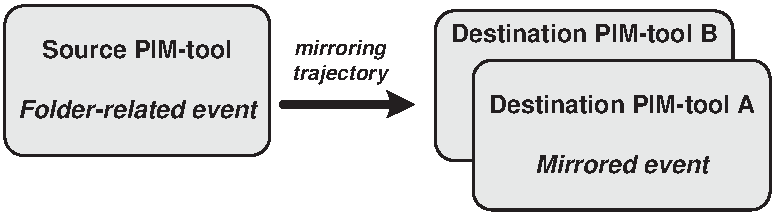
\includegraphics[height=2cm]{pictures/main-study/trajectory.pdf}
	\end{center}
	\caption{The trajectory of a mirroring event}
	\label{fig:main-study:trajectory}
\end{figure}

%%%%%%%%%%%%%%%%%%%%%%%%%%%%%%%%%%%%%%
% %%%%%%%%%%%%%%%%%%%%%%%%%%%%%%%%%%%%
% FIGURE - Sample from WET % Or a table?
% %%%%%%%%%%%%%%%%%%%%%%%%%%%%%%%%%%%%
%%%%%%%%%%%%%%%%%%%%%%%%%%%%%%%%%%%%%%
%%%%%%%%%%%%%%%%%%%%%%%%%%%%%%%%%%%%%%%%%
% TABLE OF PARTICIPANTS IN MAIN STUDY
%%%%%%%%%%%%%%%%%%%%%%%%%%%%%%%%%%%%%%%%%
\begin{table}[hbtp]
\begin{center}
\begin{footnotesize}
\setlength{\extrarowheight}{2pt}
% REMEMBER: replace _ WITH \_
% Table generated by Excel2LaTeX from sheet '5 WET sample'
\begin{tabular}{|c|p{2.5cm}|p{2cm}|p{2cm}|p{2cm}|p{2.5cm}|}
\hline
{\bf Date} & {\bf Folder event description (all are creation events)} & {\bf File system} & {\bf Email} & {\bf Bookmark} & {\bf Was folder used to store items by the end of stage 4?} \\
\hline
 12-Nov-02 & Mirror: from files to email & {\bf BOD/\underline{Meetings}} & {\it BOD/\underline{Meetings}} &    {\bf -} & Used in files (many subfolders), email (many subfolders) \\
\hline
 12-Nov-02 & Mirror: from files to email & {\bf BOD/Meetings/ \underline{TMT}} & {\it BOD/Meetings/ \underline{TMT}} &    {\bf -} & Used in files (2 subfolders), email (2 subfolders) \\
\hline
 12-Nov-02 & Mirror: from files to email & {\bf BOD/Meetings/ TMT/\underline{2002\_1113}} & {\it BOD/Meetings/ TMT/\underline{2002\_1113}} &    {\bf -} & Used in files (1 item), email (4 items) \\
\hline
 12-Nov-02 & Mirror: from files to email & {\bf BOD/Meetings/ \underline{PMC}} & {\it BOD/Meetings/ \underline{PMC}} &    {\bf -} & Used in email (1 subfolder) \\
\hline
 12-Nov-02 & Mirror: from files to email & {\bf BOD/\underline{papers}} & {\it BOD/\underline{papers}} &    {\bf -} & Used in files (6 items), email (1 item) \\
\hline
 21-Nov-02 & Not mirrored from files & {\bf BOD/WP4/ \underline{htmldocs}} &          - &    {\bf -} & Used in files (>10 items) \\
\hline
 28-Nov-02 & Mirror: from email to files and BM & {\it \underline{Context-Aware}} & {\bf \underline{Context-Aware}} & {\it \underline{Context-Aware}} & Used in files (12 items) \\
\hline
 02-Dec-02 & Mirror: from files to email & {\bf BOD/\underline{audit}} & {\it BOD/\underline{audit}} &          - & Used in files (9 items), email (12 items) \\
\hline
 02-Dec-02 & Not mirrored from files & {\bf BOD/WP4/ \underline{Mpeg7Schema}} &            - &          - & Used in files (>10 items) \\
\hline
 03-Dec-02 & Not mirrored from files & {\bf BOD/audit/ \underline{graf}} &          - &          - & Used in files (3 items) \\
\hline
 03-Dec-02 & Not mirrored from files & {\bf BOD/audit/ \underline{hutter}} &          - &          - & Used in files (3 items) \\
\hline
 04-Dec-02 & Mirror: from files to email and BM & {\bf BOD/WP4/ \underline{MPEGDocs}} & {\it BOD/WP4/ \underline{MPEGDocs}} & {\it BOD/\underline{WP4}/ \underline{MPEGDocs}} & Used in files (2 items), email (1 item) \\
\hline
 06-Dec-02 & Mirror: from email to files and BM & {\it BOD/\underline{FP6}} & {\bf BOD/\underline{FP6}} & {\it BOD/\underline{FP6}} & Used in files (3 items), email (13 items) \\
\hline
\end{tabular}  
\end{footnotesize}
\caption{Extract of the workspace evolution transcript from stage 4 for participant F2.}
\label{table:main-study:wet-example}
\end{center}
\end{table}
\normalsize



%%%%%%%%%%%%%%%%%%%%%%%%%%%%%%%%%
% FIN THESIS Chapter 6 MAIN STUDY METHOD
%%%%%%%%%%%%%%%%%%%%%%%%%%%%%%%%%